
\documentclass[12pt]{article} 
\usepackage[utf8]{inputenc}
\usepackage[slovak]{babel}
\usepackage[hidelinks,unicode = true]{hyperref}
\usepackage{outline}
\usepackage{graphicx}
\usepackage{longtable} %pro tabulky delší než jedna stránka
%\usepackage{biblatex}
%\addbibresource{literatura.bib}
\usepackage{cite}
\usepackage{caption}
%\usepackage{float} %upevneni tabulky
%\restylefloat{table}
\setcounter{secnumdepth}{3}
\setcounter{tocdepth}{3}

%===========================================================================
\begin{document}           % Konec preambule a zároveň začátek vlastního textu
\begin{titlepage}
\centering
\Large \textbf{České vysoké učení technické v Praze }\\ Fakulta stavební
\vspace{2cm}

\begin{figure}[h!] %logoCVUT
\centering
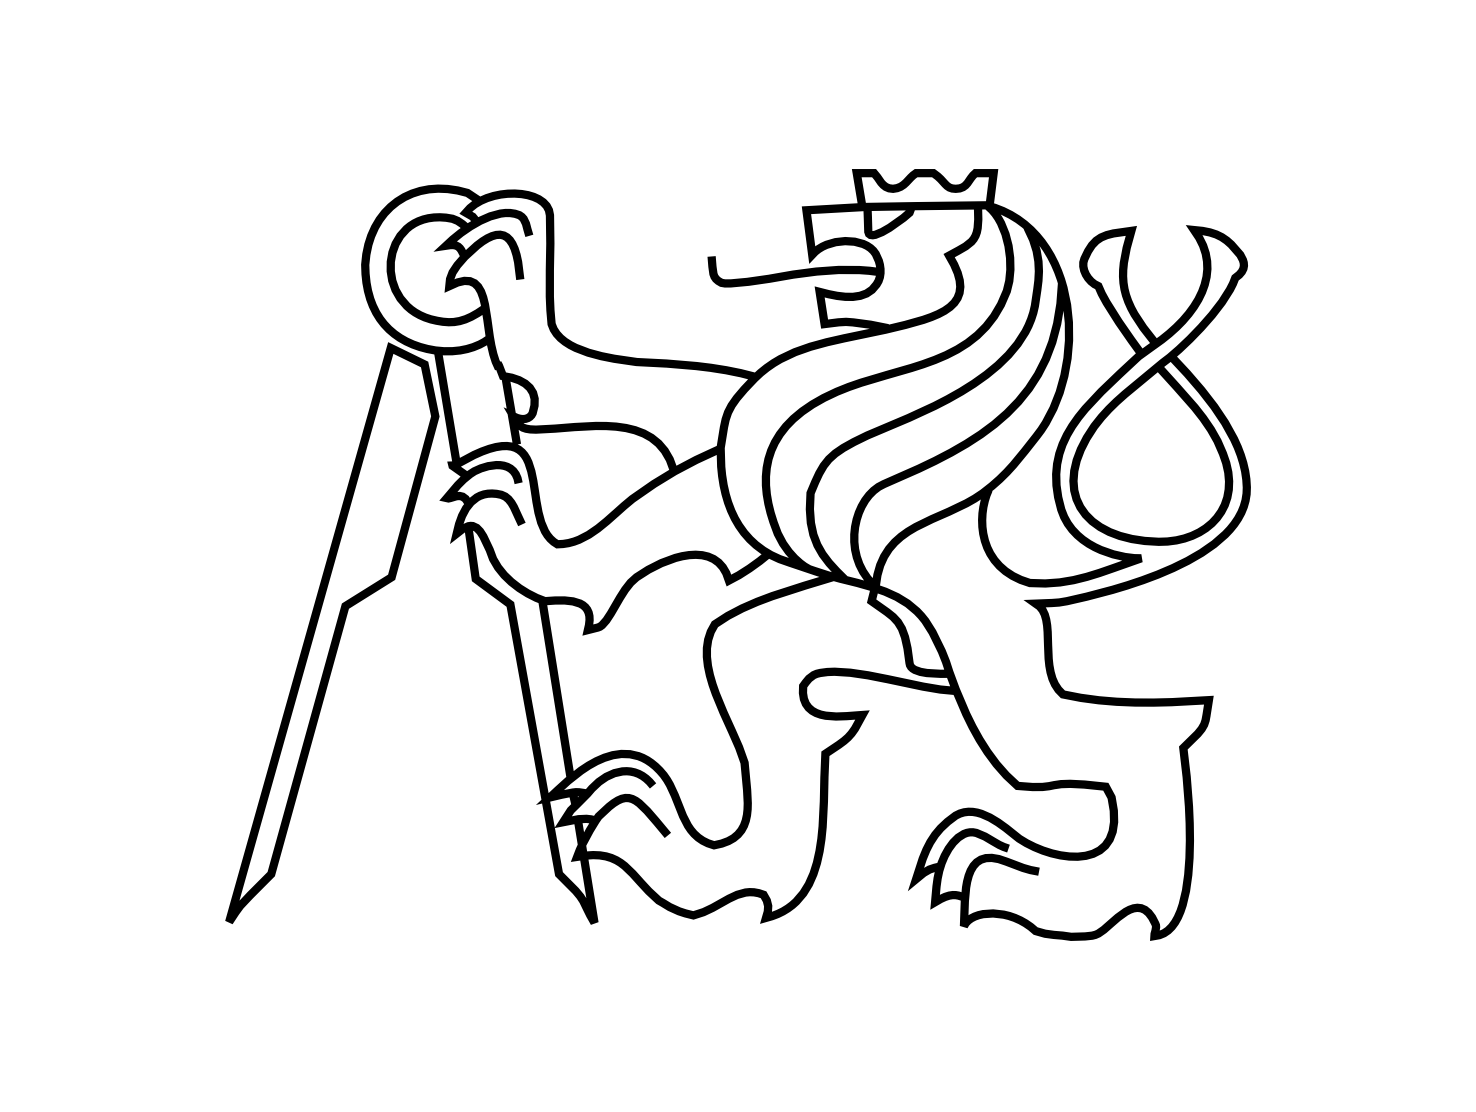
\includegraphics[width=7cm]{./img/cvut.png}
\end{figure}
 
\Large \textbf{155ADKG Algoritmy v digitální kartografii}
\vspace{1cm}

\LARGE  \textbf{Množinové operace s polygony}
\vspace{3cm}

\Large Bc. Lukáš Kettner Bc. Martin Hulín \\ 17.12.2019

 \thispagestyle{empty} %neočísluje první stránku
\end{titlepage}

\tableofcontents    % vytváří  Obsah 
\newpage %začne na nové stránce
%------------------------------------------------------------------------
\section{Zadanie}

\begin{figure}[h!]
	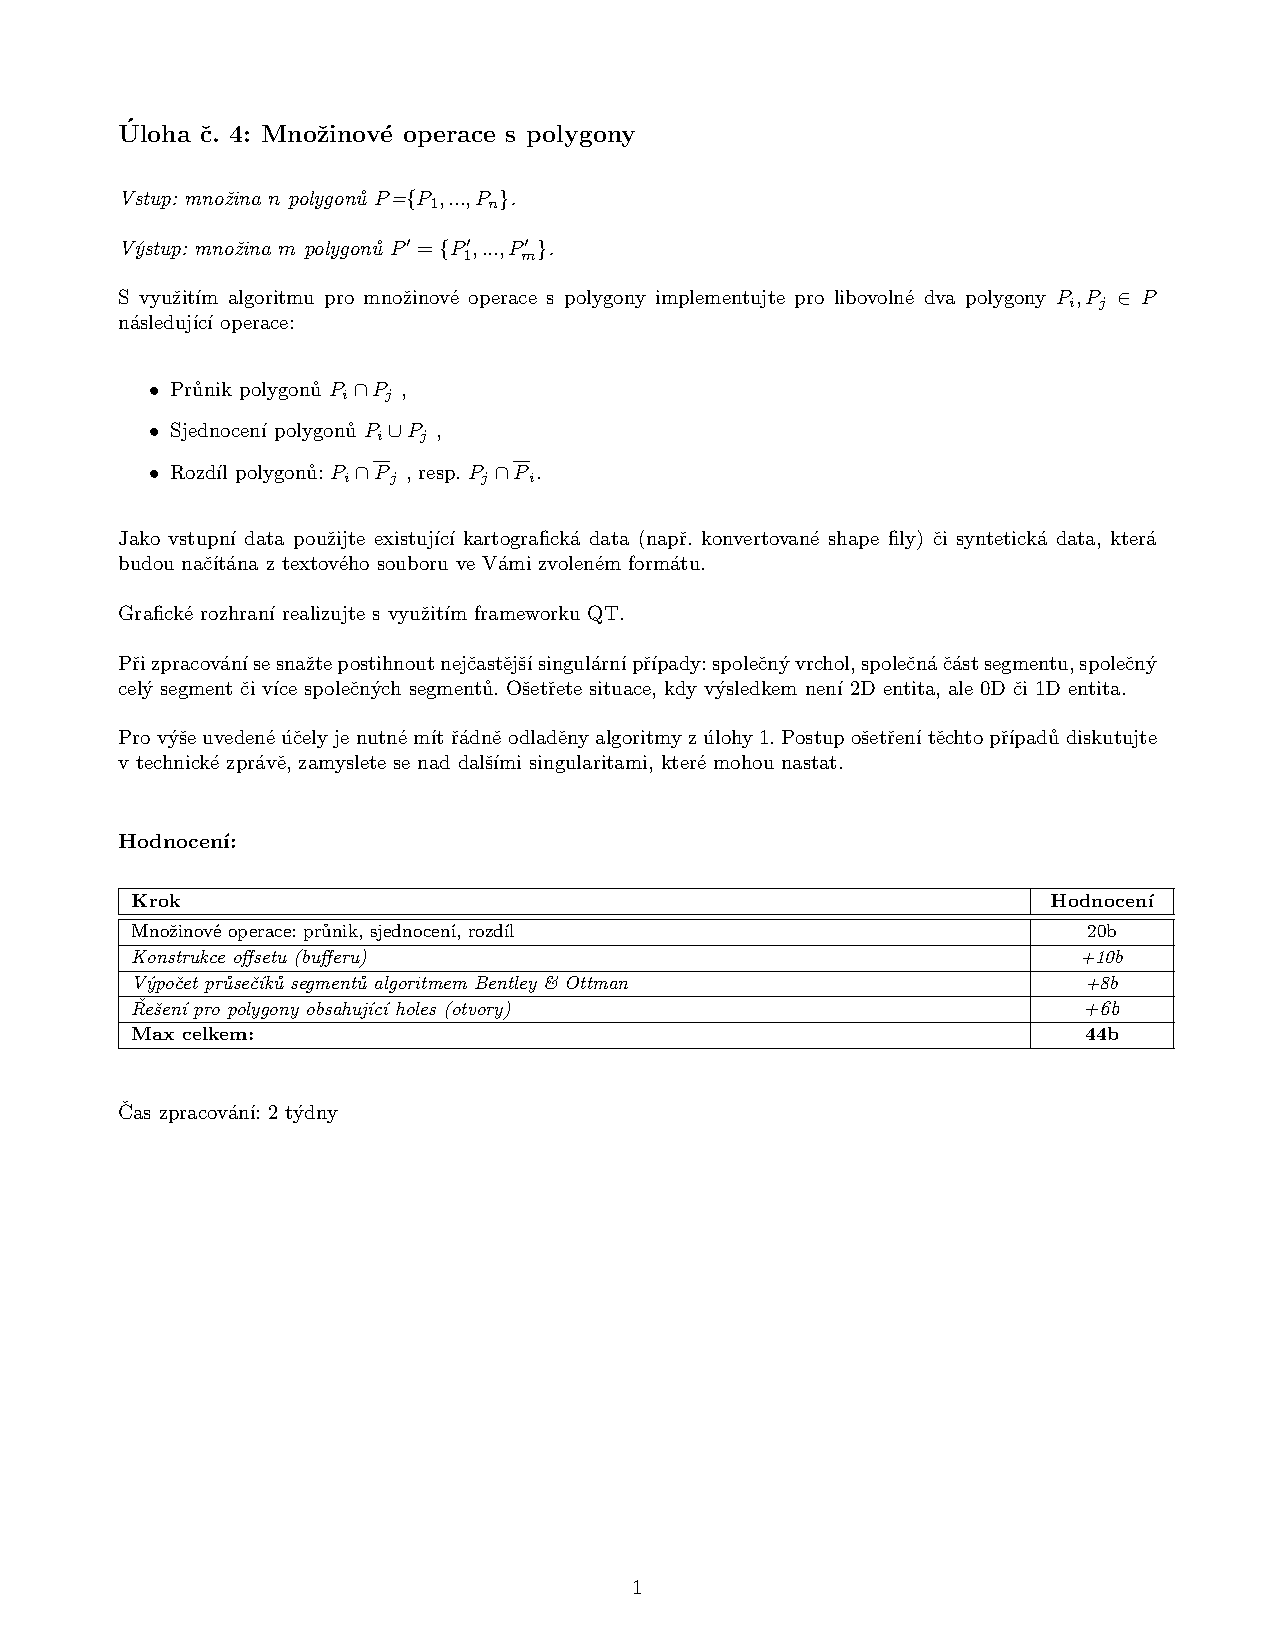
\includegraphics[clip, trim=0cm 4cm 0cm 3cm, width=1.2\textwidth]{zadani.pdf}
\end{figure}
\subsection{Bonusové úlohy}
V rámci úlohy sú vypracované tieto bonusové úlohy

\begin{itemize}
\item Riešenie pre polygóny obsahujúce otvory
\end{itemize}

%------------------------------------------------------------------------
\clearpage 
\section{Popis a rozbor problému}
Podstatou úlohy je tvorba aplikácie, v ktorej grafickom rozhraní bude možné prevádzať základné množinové operácie. V rámci úlohy sa zoberáme operáciami prienik, zjednotenie a rozdiel polygónov A a B.

\begin{center}
   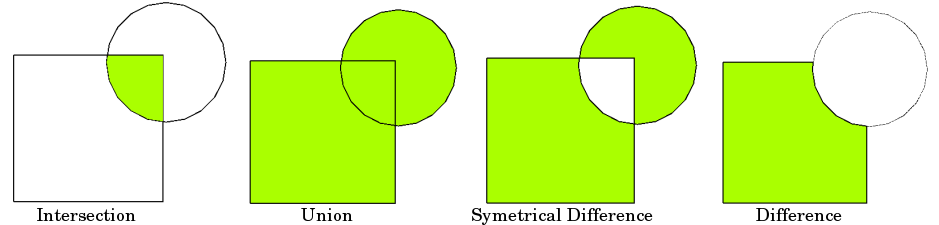
\includegraphics[width=12cm]{./img/operac.png}
   \captionof{figure}{Typy množinových operácií s polygónmi}
\end{center}
%------------------------------------------------------------------------
\clearpage 
\section {Popis použitých algoritmov}
\subsection {Výpočet priesečníkom, zotriedenie a aktualizácia}
Využili sme funkciu get2LinesPosition. Táto funkcia kontroluje hrany z polygonu A a polygonu B na existenciu priesečníku. V úlohe bol použitý datový typ QPointFB, ktorý uchováva hodnoty parametrov alfa a beta. Tento typ je odvodený od typu QPointF.  Pokiaľ priesečník existoval spočítali sme jeho súradnice. 

Pri výpočte priesečníku môžu nastať nasledujúce možnosti :
\begin{enumerate}
\item úsečky sú kolineárne
\item úsečky sú rovnobežné
\item úsečky sú rôznobežné
\item úsečky sú mimobežné
\end{enumerate}

Tieto hodnoty sa ukladajúdo datového typu map - kľúč je parameter alfa / beta,  hodnota priesečník. Priesečníky boli ďalej vložené do správneho polygónu na správnu pozíciu pomocou funkcie processIntersection.

\subsubsection {Implementácia metódy processIntersection}
\begin{enumerate}
\item Nastavenie tolerancie epsilon
\item $ if ((t >= epsilon ) \&\& (t <= 1- epsilon ) $
\item $ i += 1$
\item $polygon.insert(polygon.begin() + i,pi $ // priraď priesečník polygónu na pozíciu
\end{enumerate}

\subsubsection {Implementácia funkcie computePolygonIntersection}
\begin{enumerate}
\item Cyklus $ for ( int i = 0 ; i < pa.size(); i++)$ - prechádame celý polygón A
\item Vytvotenie map $ std::map< double, QPointFB> intersections$
\item  Cyklus $ for ( int j = 0 ; j < pb.size(); j++)$ - prechádame celý polygón B
\item \hspace {1.0cm}   $ if (get2LinesPosition(...) == INTERSECTED $ podmienka ak existuje prisečník
\item \hspace {1.5cm}  Získaj hodnoty alpha, beta, ulož priesečník do mapy na základe alpha $intersections[alpha]=p_i $
\item \hspace {1.5cm} $processIntersection(pi, beta, pb, j) $
\item \hspace {1.0cm} Ak bol nájdený aspoň jeden priesečník 
\item \hspace {1.0cm} prejdi mapu $for (std::pair<double, QPointFB> item:intersections)$
\item \hspace {1.0cm}získaj druhú hodnotu z páru  $QPointFB pi = item.second$
\item \hspace {1.0cm} $processIntersection(pi, alfa, pa, i) $
\end{enumerate}

\subsection {Ohodnotenie vrcholov}
Tento algoritmus uplatňuje ako ohodnocovacie pravidlo polohu vrcholu v polygóne voči druhému vrcholu. Rozsah hodnotenia v závislosti na polohe môže byť Inner, Outer, On. Tieto hodnoty boli uložené do nového datového typu TPointPolygonPosition. K určeniu polohy sme využili Winding Number algoritmus.

\subsubsection{Implementácia metódy setPosition}
\begin{enumerate}
\item Cyklus $ for(int i = 0; i < n; i++)$ - prechádame celý polygón A
\item Výpočet stredového bodu hrany 
\item \hspace {1.0cm} $double mx = (pa[i].x() + pa[(i + 1)\%n].x()) / 2;$
\item \hspace {1.0cm} $double my = (pa[i].y() + pa[(i + 1)\%n].y()) / 2;$
\item  Uloženie bodu $ QPointFB m(mx, my);$
\item Určenie polohy metodou Winding Number
\newline \hspace {1.0cm}   $TPointPolygonPosition position = positionPointPolygonWinding(m, pb);$
\item \hspace {1.0cm} Uloženie pozície počiatočného vrholu hrany
\end{enumerate}

\subsection {Ohodnotenie hran}
Výber hran pre množinové operácie znázorňuje nasledujúca tabuľka.

\begin{table}[h]
	\begin{tabular}{|l|l|l|}
		\hline
		Operace & A             & B             \\ \hline \hline
		$C = A\cap B$  & Inner         & Inner         \\ \hline
		$C = A\cup B$  & Outer         & Outer         \\ \hline
		$C = A\cap \overline{B}$  & Outer         & Inner         \\ \hline
		$C = B\cap \overline{A}$  & Inner         & Outer         \\ \hline
		$C = A\bigtriangleup B$  & Inner + Outer & Inner + Outer \\ \hline
	\end{tabular}
\end{table}

\subsection {Vytvorenie hran}
Vrcholy, ktorým náleží príslušne ohodnotenie sme následne spojili do hrán a uložili do vektoru, ktorý je vykreslovaný.

\subsubsection{Implementácia metódy selectEdges}
\begin{enumerate}
\item Cyklus $ for(int i = 0; i < n; i++)$  prechádzame celý polygon
\item Nájdenie vhodnej hrany
\item \hspace {1.0cm} $Edge e (pol[i], pol[(i+1)\%pol.size()]);$ vytvorenie hrany
\item \hspace {1.0cm} $edges.push_back(e);$ pridanie hrany do vektoru hran
\end{enumerate}
\clearpage 
%------------------------------------------------------------------------
\section{Vstupné dáta}
Vstupnými dátami sú dva polygóny, naklikané ručne v grafickom rozhraní aplikácie. Pomocou tlačítka PolagonA/B je možné prepínať medzi kresbou jednotlivých polygónov.

\section{Výstupné - generovanie množinových operácií}
Výstupnými dátami je graficky reprezentované zobrazenie množinových operácií.

%------------------------------------------------------------------------

\section{Ukážka vytvorenej aplikácie}

\begin{center}
   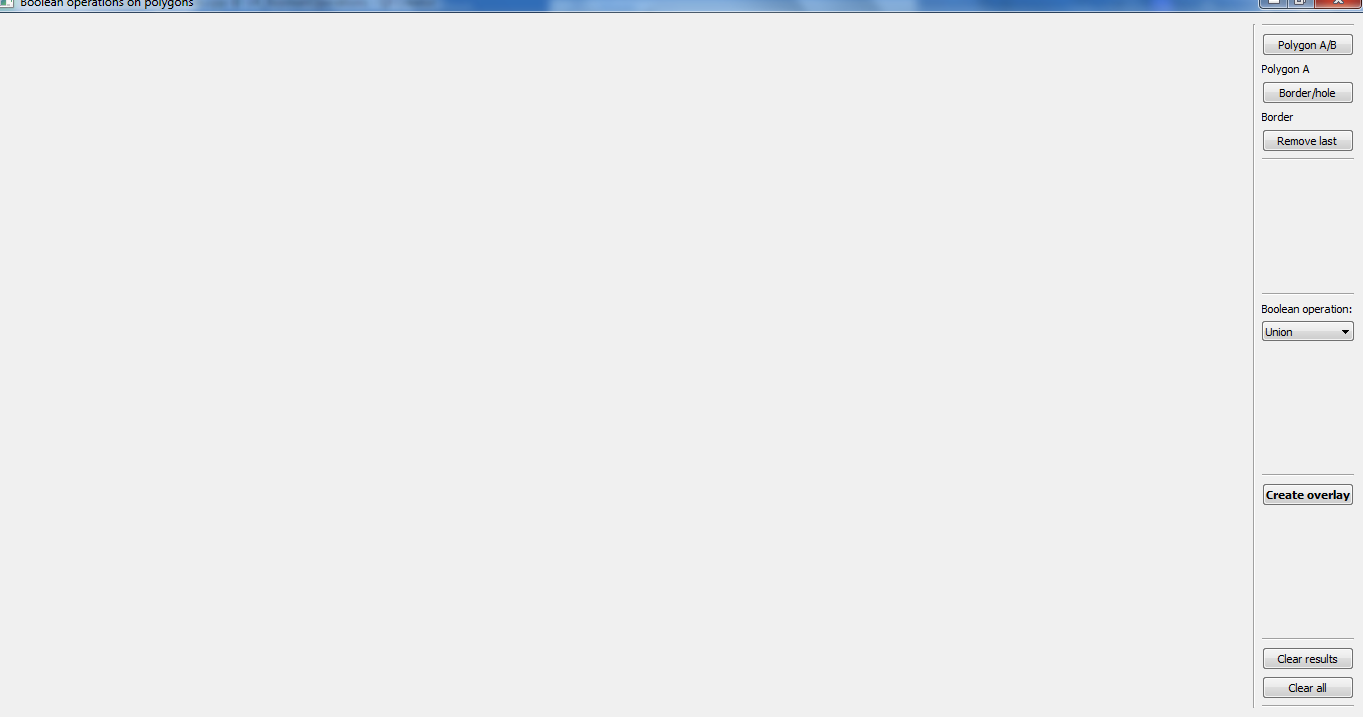
\includegraphics[width=10cm]{./img/aplikacia1.png}
   \captionof{figure}{Ukážka grafického rozhrania aplikácie}
\end{center}

\begin{center}
   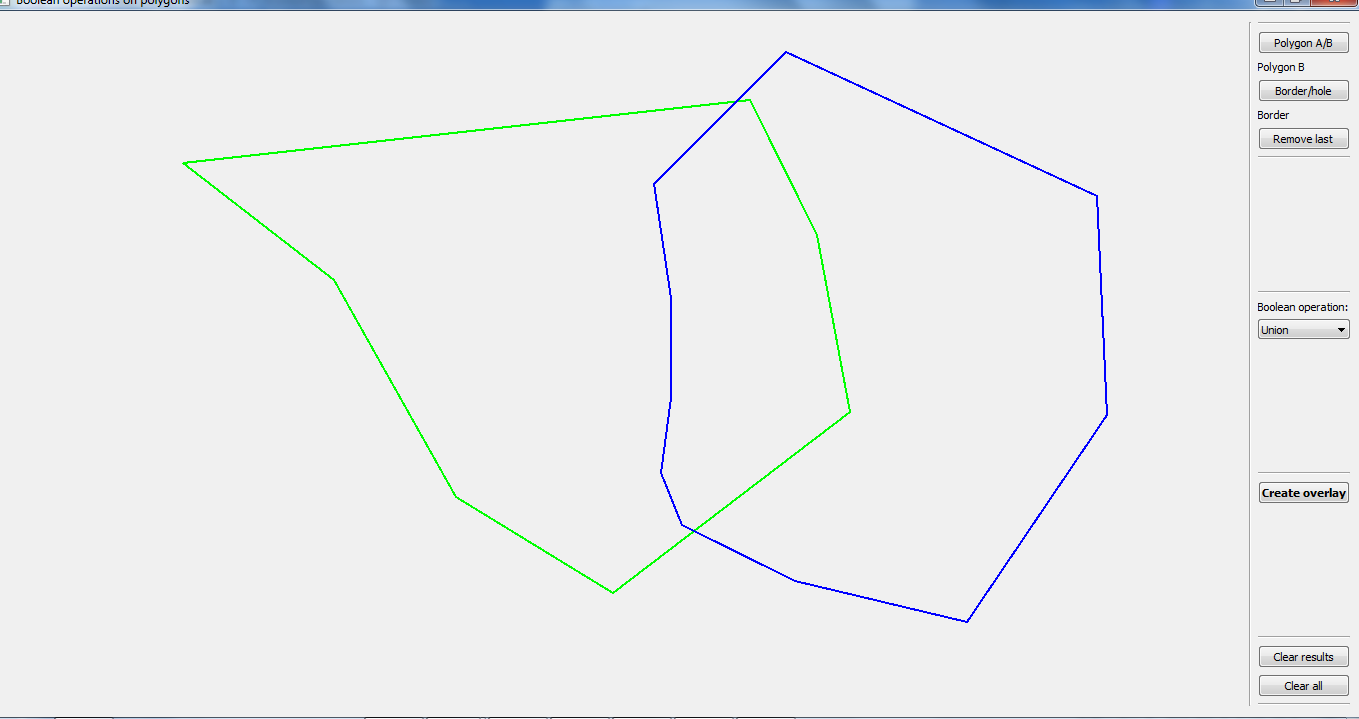
\includegraphics[width=10cm]{./img/aplikacia2.png}
   \captionof{figure}{Ukážka grafického rozhrania aplikácie - 2 polygóny}
\end{center}

\begin{center}
   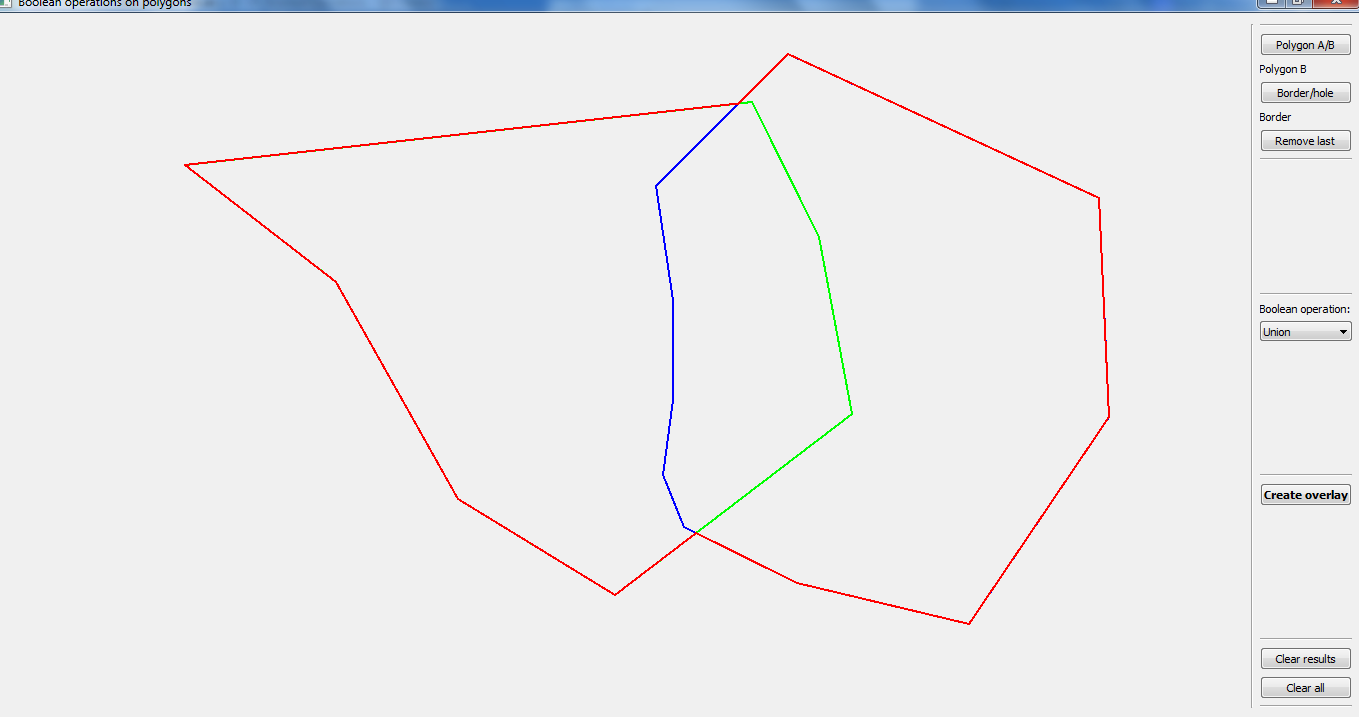
\includegraphics[width=10cm]{./img/aplikacia_union.png}
   \captionof{figure}{Ukážka grafického rozhrania aplikácie - Union}
\end{center}

\begin{center}
   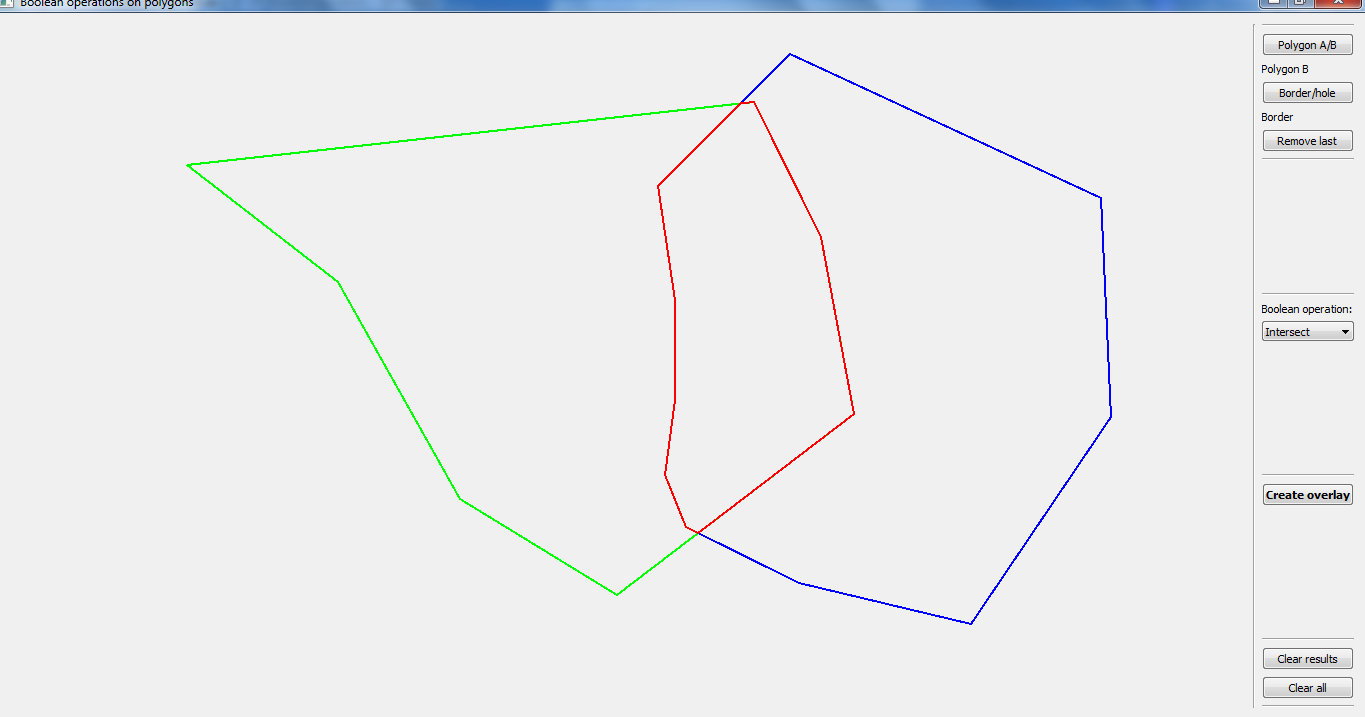
\includegraphics[width=10cm]{./img/aplikacia_intersect.png}
   \captionof{figure}{Ukážka grafického rozhrania aplikácie - Intersect}
\end{center}

\begin{center}
   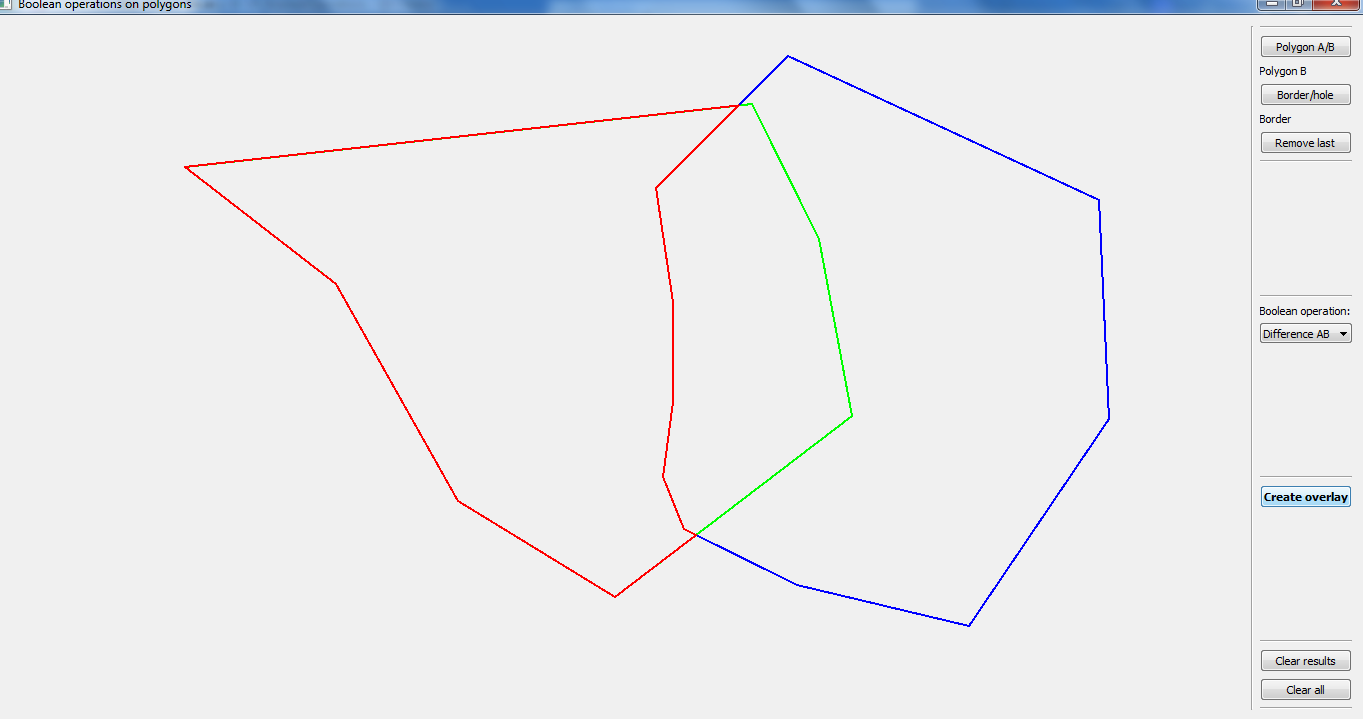
\includegraphics[width=10cm]{./img/aplikacia_AB.png}
   \captionof{figure}{Ukážka grafického rozhrania aplikácie - Difference AB}
\end{center}

\begin{center}
   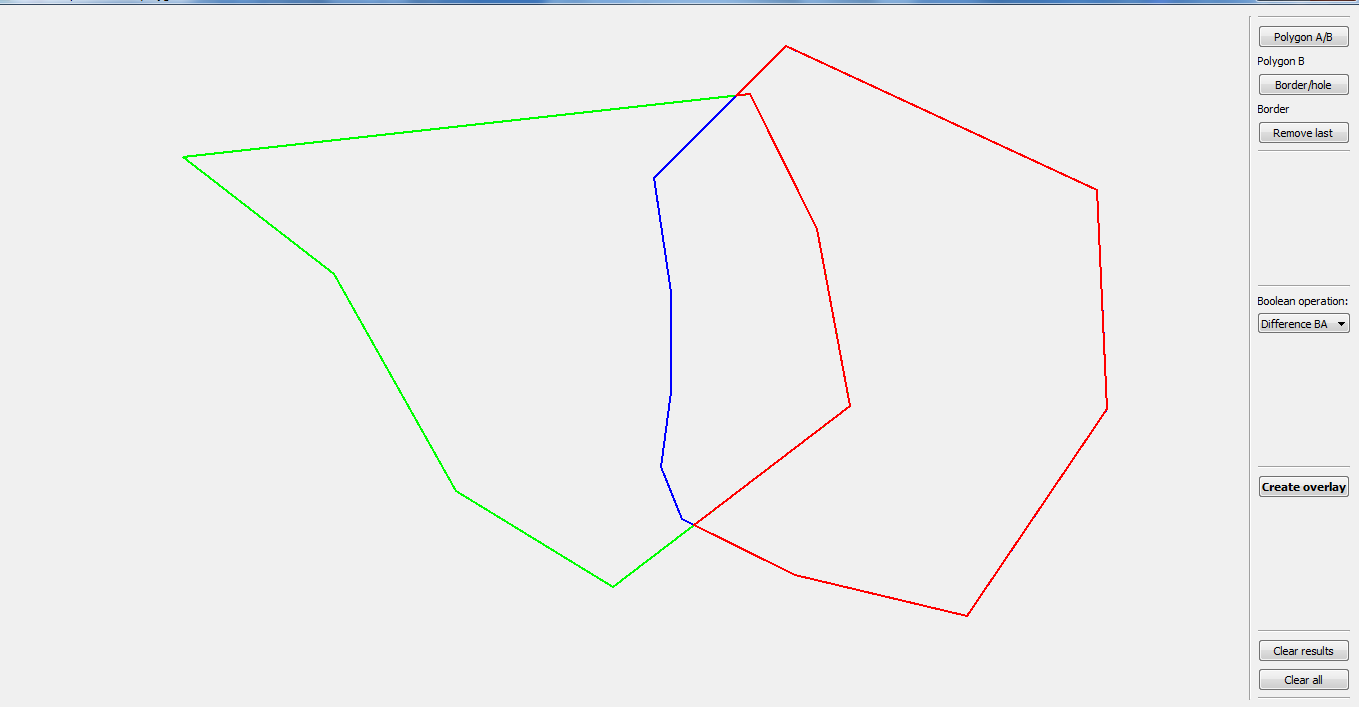
\includegraphics[width=10cm]{./img/aplikacia_BA.png}
   \captionof{figure}{Ukážka grafického rozhrania aplikácie - Difference BA}
\end{center}

\begin{center}
   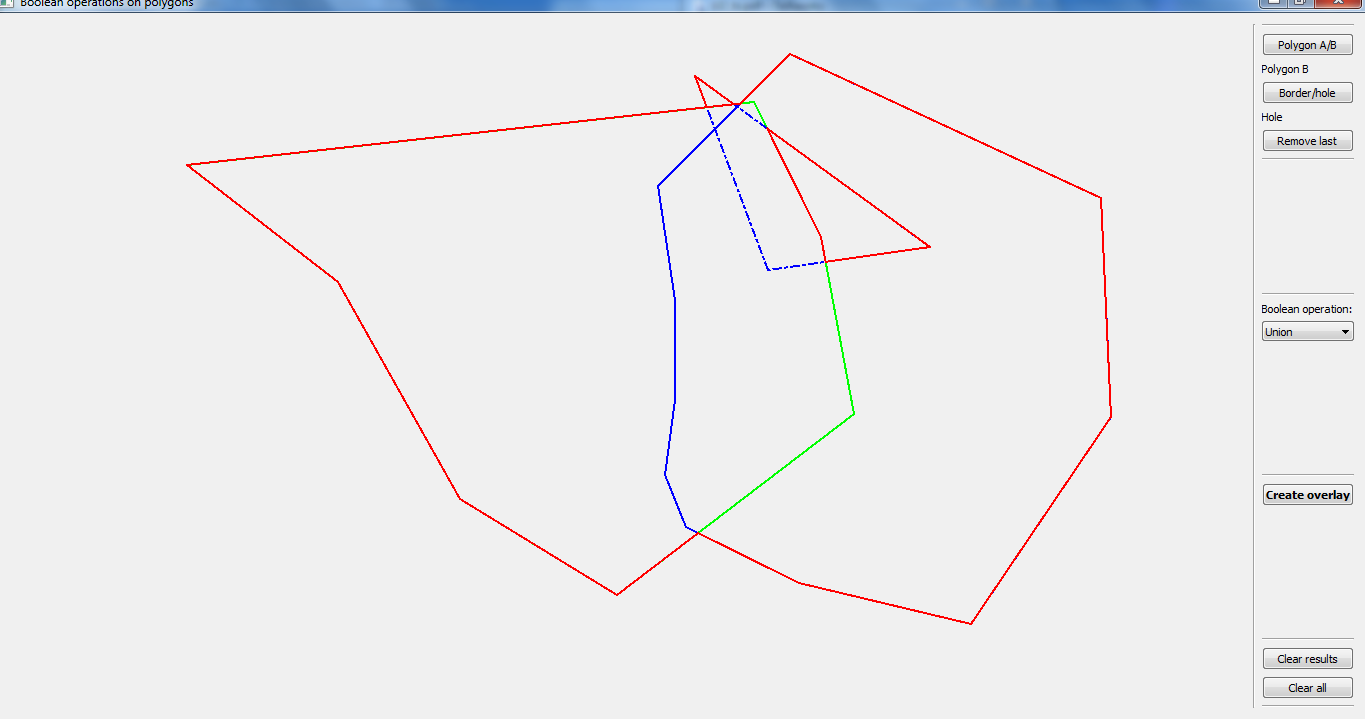
\includegraphics[width=10cm]{./img/aplikacia_diera_Union.png}
   \captionof{figure}{Ukážka grafického rozhrania aplikácie - Holes pri operácii Union}
\end{center}

%-------------------------------------------------------------------------
\section{Dokumentácia}
\subsection{Trieda Algorithms}
Triedu Algorithms sme použili pre deklarovanie funkcií pre výpočtové algoritmy tvorby množinových operácií s polygónmi.

\subsubsection{Metódy}

\begin{enumerate}
\item[] \underline{getAngle2Vectors}
\begin{itemize}
\item Slúži k určeniu uhlu medzi dvoma priamkami. Jej návratovou hodnotou je double
\item na vstupe má : súradnice bodov $p_1, p_2, p_3, p_4$ určujúcich prvú a druhú priamku
\item výstupom je hodnota uhlu medzi priamkami 
\end{itemize}

\item[] \underline{getPointLinePosition}
\begin{itemize}
\item Slúži na určenie polohy bodu voči priamke. Jej návratovou hodnotou je integer.
\item na vstupe má : súradnice určovaného bodu q , súradnice bodov priamky $p_1$ $p_2$
\item na výstupe hodnoty :
\item[] - LeftHp
\item[] - RightHp
\item[] - Colinear
\end{itemize}

\item[] \underline{positionPointPolygonWinding}
\begin{itemize}
\item slúži k určeniu polohy bodu prostredníctvom Winding Number algoritmu. Jej návratový typ je integer.
\item na vstupe má : QPointFB q – bod ktorého polohu určujeme, std$::$vector$<$QPointFB$>$ pol – polygon, voči ktorému určujeme polohu bodu q
\item výstupom je hodnota :
\item[] - Outer
\item[] - Inner
\end{itemize}

\item[] \underline{get2LinesPosition}
\begin{itemize}
\item funkcia slúžia k výpočtu polohy dvoch priavok voči sebe. 
\item na vstupe je sú body QPointFB p1, p2, p3, p4, pi
\item na výstupe hodnoty :
\item[] - Identical
\item[] - Paralel
\item[] - Intersected
\item[] - NonIntersected
\end{itemize}


\item[] \underline{booleanOperations}
\begin{itemize}
\item funkcia slúžia k prevedeniu množinových operácií.. 
\item na vstupe je sú polygóny bodov QPointFB polygonA, polygonB a typ operácie 
\item na výstupe je vektor hrán odpovedajúci zvolenej operácii pre polygóny
\end{itemize}


\item[] \underline{processIntersection}
\begin{itemize}
\item funkcia slúžia k prevedeniu zaradenia vypočítaného priesečníku na správnu pozíciu v príslušnom polygóne. Jej návratovym typom je void. 
\end{itemize}


\item[] \underline{computePolygonIntersection}
\begin{itemize}
\item funkcia slúžia k výpočtu priesečníku. Jej návratovym typom je void. 
\end{itemize}


\item[] \underline{setPositionsAB}
\begin{itemize}
\item funkcia je pomocnou funkciou pre boolenOperations. Jej návratovym typom je void. 
\end{itemize}


\item[] \underline{setPositions}
\begin{itemize}
\item funkcia slúži k určeniu pozície hrany. Jej návratovym typom je void. 
\end{itemize}


\item[] \underline{selectEdges}
\begin{itemize}
\item funkcia slúži k vybraniu príslušných hrán. Jej návratovym typom je void. 
\end{itemize}


\item[] \underline{booleanOperationsHoles}
\begin{itemize}
\item funkcia slúžia k prevedeniu množinových operácií pri zadaní Holes. 
\item na vstupe je sú polygóny bodov QPointFB polygonA, polygonB a typ operácie 
\item na výstupe je vektor hrán odpovedajúci zvolenej operácii pre polygóny
\end{itemize}


\item[] \underline{mergeVectors}
\begin{itemize}
\item funkcia slúži k zlúčeniu vektorov hrán. Jej návratovym typom je void. 
\end{itemize}
\end{enumerate}

\subsection{Trieda Draw}
Trieda Draw slúži ku grafickému vykresleniu množinových operácií.

\subsubsection{Členské premenné}
\begin{enumerate}

\item[] \underline {std::vector}$<${QPointFB}$>${a, b}
\begin{itemize}
\item vektory bodov, ktoré tvoria  jednotlivé polygóny A a B. Polygón A sa vykresluje plnou čiarou zelenej farby, polygon B plnou čiarou modrej farby.
\end{itemize}

\item[] \underline {std::vector}$<${QPointFB}$>${inA, inB}
\begin{itemize}
\item vektory bodov, ktoré tvoria diery v jednotlivých polygónoch. U každého polygónu je možná len jedna diera. Diery sa vykreslujú rovnakou farbou ako polygóny, no čiarkovanou čiarou.
\end{itemize}

\item[] \underline {std::vector}$<${Edge}$>${res}
\begin{itemize}
\item je to vektor, ktorý obsahuje hrany tvoriace výsledok množinovej operácie. Tá je vykreslená červenou farbou.
\end{itemize}

\item[] \underline {std::vector}$<${Edge}$>${removeEdges}
\begin{itemize}
\item je to vektor, ktorý obsahuje hrany, ktoré majú byť vo výsledku zakryté / zafarbené. Ich vykreslenie je prevedené bilou farou, čo je mierne vidieť ale v rámci praktického použitia to bolo najjednoduchšie možné riešenie. 
\end{itemize}

\item[] \underline {bool ab}
\begin{itemize}
\item táto premenná indikuje v akom bode je kreslenie, či užívateľ kreslí polygón A alebo B. V deafault nastavení sa kreslí polygon A.
\end{itemize}

\item[] \underline {bool inout}
\begin{itemize}
\item premenná indikuje kreslenie hranice / diery. Defaultne nastavenie je kresba hranice.
\end{itemize}
\end{enumerate}

\subsubsection{Metódy}
\begin{enumerate}
\item[] \underline{paintEvent}
\begin{itemize}
\item slúži k vykresleniu naklikaných hran v tvare polygónov. Návratovým typom je void.
\end{itemize}
\item[] \underline{void mousePressEvent}
\begin{itemize}
\item slúži k vykresleniu bodu  stlačením tlačidla myši, v okamihu stlačenia tlačidla na myši sa uložia súradnice bodu. Návratovým typom je void.
\end{itemize}
\item[] \underline{void drawPolygon}
\begin{itemize}
\item slúži k vykresleniu polygónu. Návratovým typom je void.
\end{itemize}
\item[] \underline{void clearResult}
\begin{itemize}
\item slúži k vymazaniu výsledku vykonanej množinovej operácie. Návratovým typom je void.
\end{itemize}
\item[] \underline{void removeLast}
\begin{itemize}
\item slúži k vymazaniu poslednej pridanej hrany polygónu. Návratovým typom je void.
\end{itemize}
\item[] \underline{void clearAll}
\begin{itemize}
\item slúži k vymazaniu obsahu celého grafického okna aplikácie. Návratovým typom je void.
\end{itemize}

\item[] \underline{getA}
\begin{itemize}
\item slúži k vráteniu členskej premennej a
\end{itemize}

\item[] \underline{getB}
\begin{itemize}
\item slúži k vráteniu členskej premennej b
\end{itemize}

\item[] \underline{getAHole}
\begin{itemize}
\item slúži k vráteniu členskej premennej inA
\end{itemize}

\item[] \underline{getBHole}
\begin{itemize}
\item slúži k vráteniu členskej premennej inB
\end{itemize}

\item[] \underline{getRes}
\begin{itemize}
\item slúži kvráteniu členskej premennej res
\end{itemize}

\item[] \underline{getRemoveEdges}
\begin{itemize}
\item slúži k vráteniu členskej premennej removeEdges
\end{itemize}

\item[] \underline{bool getPolygonStatus}
\begin{itemize}
\item slúži k vráteniu členskej premennej ab
\end{itemize}

\item[] \underline{bool getDrawStatus}
\begin{itemize}
\item slúži k vráteniu členskej premennej inout
\end{itemize}

\item[] \underline{setA}
\begin{itemize}
\item slúži k nastaveniu členskej premennej a
\end{itemize}
\item[] \underline{setB}
\begin{itemize}
\item slúži k nastaveniu členskej premennej b
\end{itemize}
\item[] \underline{setRes}
\begin{itemize}
\item slúži k nastaveniu členskej premennej res
\end{itemize}
\item[] \underline{setRemoveEdges}
\begin{itemize}
\item slúži k nastaveniu členskej premennej removeEdges
\end{itemize}
\item[] \underline{void changePolygon}
\begin{itemize}
\item slúži k zmene polygónu pri vykreslovaní
\end{itemize}
\end{enumerate}

\subsection{Trieda Edge}
Je to definície datového typu Edge. Reprezentuje usporiadanú dvojicu vrcholov, ktoré tvoria hranu.

\subsection{Trieda QPointFB}
Je to odvodená trieda od triedy QPointF. Pridali sme k nej hodnotu parametru alpha/beta. 

\subsection{Trieda Types}
Tieda Types slúži pre definovanie nových datových typov, ktoré nám umožnili ľahšiu a prehladnejšiu implementáciu algoritmov.

\subsection{Trieda Widget}
Tieda Widget obashuje metódy ktoré sú odkazom na sloty umožňujúce vykonávať príkazy z grafického rozhrania aplikácie. Nemajú žiadne vstupné hodnoty, návratovým typom je void.

\subsubsection{Metódy}
\begin{enumerate}
\item[] \underline{on\_pushButton\_switch\_clicked}
\begin{itemize}
\item tlačidlo \textbf{Polygon A/B} po kliknutí naň sa zmení vykreslovanie polygonu A na B a opačne
\end{itemize}

\item[] \underline{on\_pushButton\_createOverlay\_clicked}
\begin{itemize}
\item tlačidlo \textbf{Create overlay}  po kliknutí naň sa vygeneruje zvolená množinová operácia
\end{itemize}

\item[] \underline{on\_pushButton\_clearResult\_clicked}
\begin{itemize}
\item tlačidlo \textbf{Clear result}  po kliknutí naň sa vymaže výsledok množinovej operácie
\end{itemize}
\item[] \underline{on\_pushButton\_clearAll\_clicked}
\begin{itemize}
\item tlačidlo \textbf{Clear all}  po kliknutí naň sa vymaže celé grafické okno Canvasu
\end{itemize}
\item[] \underline{on\_pushButton\_changeInOut\_clicked}
\begin{itemize}
\item tlačidlo \textbf{Border / Holel}  kliknutím naň je možné meniť kresbu polygónu / hole
\end{itemize}
\item[] \underline{on\_pushButton\_removeLast\_clicked}
\begin{itemize}
\item tlačidlo \textbf{Removel lastl}  kliknutím naň sa odstráni posledná vytvorená hrana
\end{itemize}
\end{enumerate}

%-------------------------------------------------------------------------

\clearpage
\section{Záver}
Výsledkom úlohy je funkčná aplikácia a grafická prezentácia množinových operácií. V aplikácii je zakomponovaná tvorba dier (holes). Hrany, ktoré majú byť vo výsledku skyté sú vykreslované bielou farbou, čo si pozorný užívateľ aplikácie určite všimne. Bohužiaľ vzhľadom na časové možnosti autorov bola táto možnosť najvhodnejším možným riešením. Tento bod je určite námetom na vylepšenie aplikácie, kedy by hrany, ktoré nemajú byť vykreslované boli vyhľadané a odstránené.

%-------------------------------------------------------------------------

\newpage
%-------------------------------------------------------------------------

%Zobrazeni seznamu obrazku
%\cleardoublepage
%\addcontentsline{toc}{chapter}{\listfigurename}
\listoffigures

%-------------------------------------------------------------------------    
\end{document}             % Konec dokumentu.
